\documentclass{beamer}

\usepackage{amsmath,amsthm, amssymb, latexsym}

\newcommand{\ts}{\textsuperscript}
\newcommand{\T}{\frac{\theta}{2}}

% Theme stuff
\usetheme{Madrid}
\useinnertheme{circles}

% Define colors
\definecolor{color0}{RGB}{0,0,0} % black, for text
\definecolor{color1}{RGB}{128,0,0} % maroon, for titles, blocks
\definecolor{color2}{RGB}{118,118,118} % dark grey, for blocks
\definecolor{color3}{RGB}{255,253,250} % background color, white
\definecolor{color4}{RGB}{214,214,206} % light grey, title backgrounds
% Set colors for basic beamer elements
\setbeamercolor{headline}{bg=color4}
\setbeamercolor{footline}{bg=color4}
\setbeamercolor{block title}{bg=color4,fg=color1}
\setbeamercolor{frametitle}{bg=color4,fg=color1}
\setbeamercolor{title}{bg=color4,fg=color1}

\title[quant gen fun]{Neutral quantitative genetic variation in structured populations}
\author{Evan Koch}
\date{September 23, 2016}
\begin{document}
\frame{\titlepage}

\begin{frame}{Is spatial variation in quatitative traits adaptive?}
\framesubtitle{{\small Fabian et al. 2015}}
  \includegraphics[width=\textwidth]{fly_size.png}
\end{frame}

\begin{frame}{Population structure can take different forms}
  \framesubtitle{{\small Petkova et al. 2015, Freedman et al. 2014}}
  \begin{columns}
    \begin{column}{.5\columnwidth}
      \includegraphics[width=\textwidth]{elephants.png}
    \end{column}
    \begin{column}{.5\columnwidth}
      \includegraphics[width=\textwidth]{dogs.png}
    \end{column}
  \end{columns}
\end{frame}

\begin{frame}{How can we describe phenotypic variation in a sample?}

  \begin{center}
    \includegraphics[width=.65\textwidth]{tree.pdf}
  \end{center}
\end{frame}

\begin{frame}{Probability distribution $\Leftrightarrow$ moment generating function (MGF)}
  \begin{equation}
    \label{eq:indivs}
    \mathbf{Y}=\{Y_a,Y_b,Y_c\}
  \end{equation}

  \begin{equation}
    \varphi_{\mathbf{Y}}(\mathbf{k}) = E\left[ e^{\mathbf{k} \cdot \mathbf{Y}} \right] =
    \int e^{\mathbf{k} \cdot \mathbf{Y}} P(\mathbf{Y}=\mathbf{y}) d\mathbf{y} \nonumber 
  \end{equation}
\end{frame}

\begin{frame}{Phenotypic MGF can be obtained from genealogy MGF}
  \framesubtitle{Compound poisson process on a tree, {\small Schraiber and Landis 2015}}
  \begin{equation}
    \label{eq:genealogy}
    \mathbf{T}=\{T_a,T_b,T_c,T_{a,b},T_{a,c},T_{b,c}\}
  \end{equation}
  \begin{equation}
    \label{eq:sub}
    \varphi_{\mathbf{T}}(\mathbf{s})\Bigr|_{s_{\omega}=\frac{\theta}{2} \left( \psi\left(\sum_{a \in \omega}k_{a}\right) -1 \right)} \nonumber 
  \end{equation}
  $\psi$ is the generating function of the mutational distribution.
\end{frame}

\begin{frame}{This becomes complicated very quickly}
  \framesubtitle{{\small Lohse et al. 2011}}
  \small
  \begin{align}
    \varphi_{\mathbf{Y}}^{\Omega}(\mathbf{k}) &=
                                                \left( \sum_{i=1}^M \binom{|\Omega_i|}{2}\eta_i  + \sum_{(i,j:i \neq j)} m_{i,j}|\Omega_i| -
                                                \sum_{i=1}^M \sum_{\omega \in \Omega_i} \T\left( \psi\left(\sum_{a \in \omega}k_{a}\right) -1\right)\right)^{-1} \nonumber \\ 
                                              &\times \left( \sum_{i=1}^M \eta_i \sum_{(a,b) \in \Omega_i:a \neq b}
                                                \varphi_{\mathbf{Y}}^{\Omega(i:a \cup b)}(\mathbf{k}) + 
                                                \sum_{(i,j):i\neq j}m_{i,j}\sum_{\omega \in \Omega_i} \varphi_{\mathbf{Y}}^{\Omega\left( i :-\omega, j: + \omega \right)}(\mathbf{k})\right) \nonumber 
  \end{align}
  \normalsize
\end{frame}

\begin{frame}{The infinitesimal limit}
  \begin{itemize}
  \item Number of loci gets big
  \item Effect of each locus gets small
  \end{itemize}
  Let the variance of mutational effects be: $Var[U]:=\tau^2$
  \begin{equation}
    \label{eq:lim}
    \lim_{L \to \infty}\tau^2L \to \sigma^2 \nonumber
  \end{equation}
  \begin{equation}
    \label{eq:lim2}
    \lim_{L \to \infty}E[U^k]L \to 0 \nonumber 
  \end{equation}
  for $k>2$.
\end{frame}

\begin{frame}{Differences become multivariate normal}
  All that matters are pairwise coalescent times.
  \begin{equation}
    \label{eq:mean}
    E[Y_1-Y_2]=0
  \end{equation}
  \begin{equation}
    \label{eq:covcoal}
    Cov[Y_1-Y_2,Y_3-Y_4] \propto E[t_{1,4}] + E[t_{2,3}] - E[t_{1,3}] - E[t_{2,4}] \nonumber
  \end{equation}
\end{frame}

\begin{frame}{Phenotypic divergence can be summarized using $Q_{ST}$}
  \begin{equation}
    \label{eq:qst}
    Q_{ST} = \frac{V_{between}}{V_{within}+V_{between}} \nonumber 
  \end{equation}
  Can derive the sampling distribution using the previous theory. 
\end{frame}

\begin{frame}{Example $Q_{ST}$ sampling distributions}
  \begin{center}
    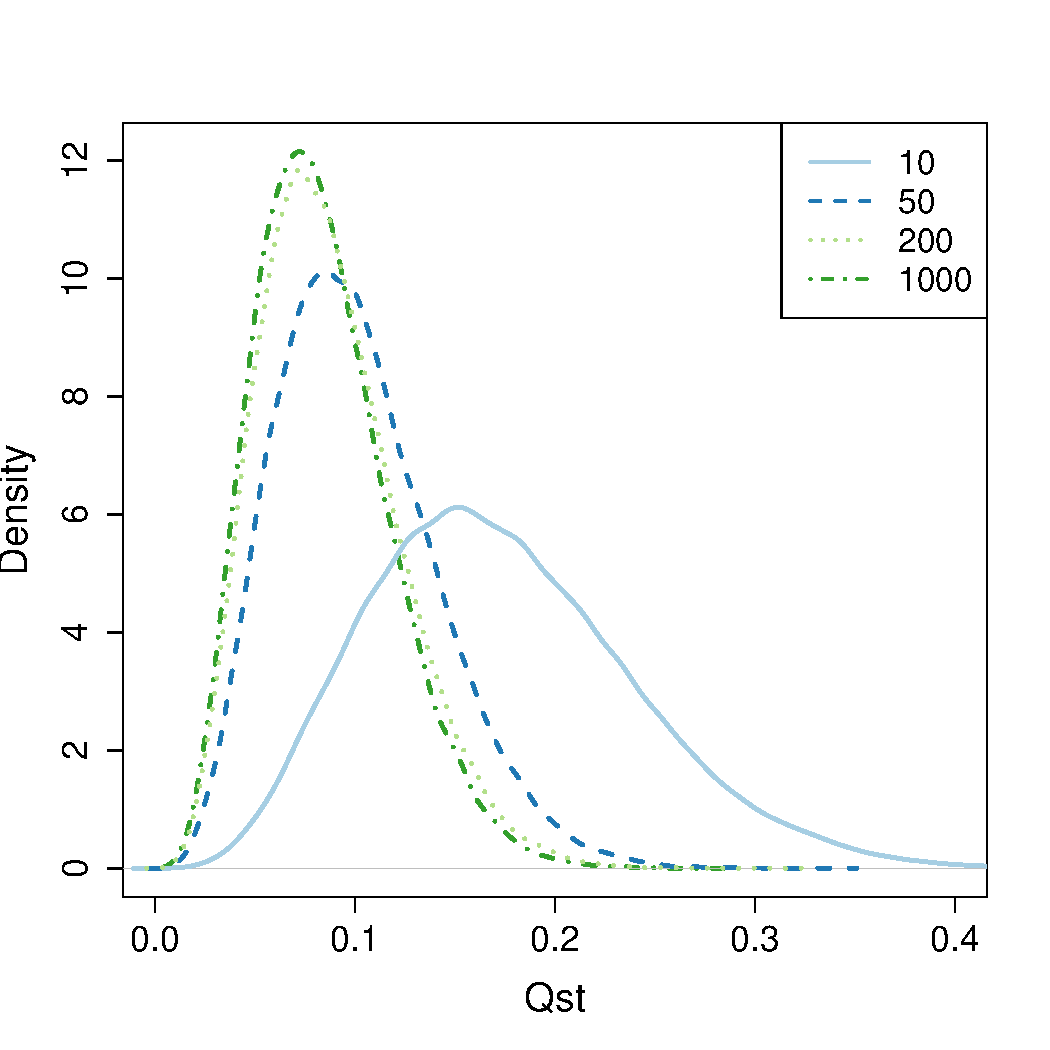
\includegraphics[width=.65\textwidth]{Qst_test.pdf}
  \end{center}
\end{frame}

\end{document}